\documentclass[12pt, paper=a4]{article}
\usepackage[utf8]{inputenc}
\usepackage[german]{babel}
\usepackage{mathrsfs}
\usepackage{amsmath}
\usepackage{amssymb}
\usepackage{listings}
\usepackage{graphicx}
\usepackage{fancyhdr}

\setlength{\parindent}{0pt}

\author{Mareike G\"ottsch, 6695217, Gruppe 2\\Paul H\"olzen, 6673477, Gruppe 1\\Sven Schmidt, 6217064, Gruppe 1}

\title{FGI 2 Hausaufgaben 7}

\rhead{M. G\"ottsch, G-2; P. H\"olzen, G-1; S. Schmidt, G-1}
\pagestyle{fancy}
\begin{document}
\maketitle

\section*{Aufgabe 7.3}
\subsection*{1.}
\begin{figure}[h!]
\centering
\includegraphics[scale=0.6]{Erreichbarkeitsgraph7-3-1.pdf}
\caption{Erreichbarkeitsgraph}
\end{figure}

\subsection*{2.}
$p_2p_4 \overset{t_3}{\rightarrow} p_1^2p_3^2 \overset{t_1}{\rightarrow} p_1p_2p_3
\overset{t_2}{\rightarrow} p_2p_4 \overset{t_3}{\rightarrow} p_1^2p_3^2 \overset{t_1}{\rightarrow} p_1p_2p_3 \overset{t_2}{\rightarrow} p_2p_4 \overset{t_3}{\rightarrow} p_1^2p_3^2$\\

\subsection*{3.}
Das Netz ist nicht verklemmungsfrei, da für die Markierung $m_1 = p1(0)p2(2)p3(0)p4(0)$ bzw. $m_2 = p1(0)p2(0)p3(0)p4(2)$ keine Transition mehr schalten kann. Aus diesem Grund ist das Netz auch nicht lebendig. Auch die Reversibilität ist nicht gegeben, da in den verklemmten Markierungen auch kein Pfad existiert, der die Anfangsmarkierung wiederherstellen könnte.\\

\subsection*{4.}
\begin{align*}
\begin{pmatrix}
0 \\ 1 \\ 0 \\ 1
\end{pmatrix}
\overset{t_3}{\rightarrow}
\begin{pmatrix}
2 \\ 0 \\ 2 \\ 0
\end{pmatrix}
\overset{t_1}{\rightarrow}
\begin{pmatrix}
1 \\ 1 \\ 1 \\ 0
\end{pmatrix}
\overset{t_2}{\rightarrow}
\begin{pmatrix}
0 \\ 1 \\ 0 \\ 1
\end{pmatrix}
\overset{t_3}{\rightarrow}
\begin{pmatrix}
2 \\ 0 \\ 2 \\ 0
\end{pmatrix}
\overset{t_1}{\rightarrow}
\begin{pmatrix}
1 \\ 1 \\ 1 \\ 0
\end{pmatrix}
\overset{t_2}{\rightarrow}
\begin{pmatrix}
0 \\ 1 \\ 0 \\ 1
\end{pmatrix}
\overset{t_3}{\rightarrow}
\begin{pmatrix}
2 \\ 0 \\ 2 \\ 0
\end{pmatrix}
\end{align*}

\subsection*{5.}
Durch Löschen der Transition $t_2$ und hinzufügen ihrer Kanten zu $t_1$ entsteht das Netz in Abbildung 2. Der Erreichbarkeitsgraph ist in Abbildung 3 zu sehen. Es ist reversibel, da von jeder erreichbaren Markierung ein Pfad existiert, der die Startmarkierung wiederherstellt. Da nur zwei Markierungen erreichbar sind ist dies leicht am Erreichbarkeitsgraphen nachvollziehbar.\\
Das Netz besitzt außerdem noch die beiden Eigenschaften Lebendigkeit und Verklemmungsfreiheit. Es ist lebendig, da über den Pfad der das Netz in die Startmarkierung zurücksetzt auch jede Transition wieder schalten kann. Es ist verklemmungsfrei, da aus jeder erreichbaren Markierung mindestens eine Transition schalten kann.\\

\begin{figure}[h!]
\centering
\includegraphics[scale=0.9]{reversible.pdf}
\caption{Reversibles Netz}
\end{figure}

\begin{figure}[h!]
\centering
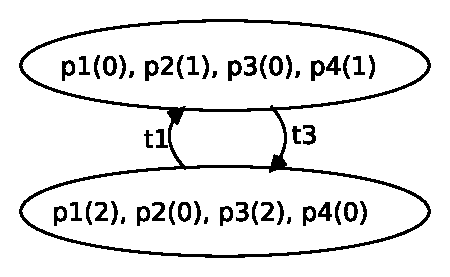
\includegraphics[scale=0.7]{Erreichbarkeitsgraph7-3-5.pdf}
\caption{Reversibles Netz}
\end{figure}

\newpage
\section*{Aufgabe 7.4}
\subsection*{1.}
Jedes reversible P/T-Netz ist lebendig.
\begin{itemize}
	\item Wahr.
	\item Falsch.
\end{itemize}
\subsection*{2.}

Wenn N ein lebendiges Netz ist und für alle Transitionen die Fortschrittseigenschaft
gilt, dann sind alle Prozesse, welche die Fortschrittseigenschaft respektieren,
unendlich.
\begin{itemize}
	\item Wahr.
	\item Falsch.
\end{itemize}

\section*{Aufgabe 7.5}
\subsection*{1.}
Der erste und gröbste Aufbau der Autoproduktion ist in Abbildung 4 zu sehen. Dabei modelliert die Transition $t_1$ Aufträge, die von Großabnehmern aufgegeben werden und als Marken auf einen Platz gelegt werden. Transition $t_2$ stellt den Mitarbeiter dar, der die Aufträge in ein Fach legt, $t_3$ den Mitarbeiter, der die Aufträge an den Lieferanten weitergibt, der durch $t_4$ modelliert ist. Der Lieferant liefert Material für 100 PKWs in ein Lager, repräsentiert durch 100 Marken, die auf einen Platz gelegt werden. Die Transition $t_5$ symbolisiert den Fertigungsprozess und legt fertige Autos in Form von Marken auf einen Platz, der wiederum als Lager dient, aus dem der Spediteur dann immer 100 Wagen auf einmal abholt.\\

Das Netz ist nebenläufig, da die Transition $t_1$ immer und unabhängig von allen anderen schalten kann. Es ist außerdem lebendig, da $t_1$ immer mehr Marken erzeugen kann und damit eine Schaltfolge existiert, mit der alle Transitionen geschaltet werden können. Das Netz ist deterministisch in dem Sinne, dass das Schalten einer Transition nur ein mögliches Ergebnis hat und es für eine einzelne Marke (bei einmaligem Schalten von $t_1$) genau eine Schaltfolge $t_1t_2t_3t_4t_5t_6$ gibt, bei der alle Transitionen einmal geschaltet werden. Das Netz ist unbeschränkt, da mit wiederholtem Schalten von $t_1$ beliebig viele Marken generiert werden können, dennoch ist es rücksetzbar, da mit der Transition $t_6$ alle Marken wieder vernichtet werden können, sodass die Startmarkierung entsteht.\\

\begin{figure}[h!]
\centering
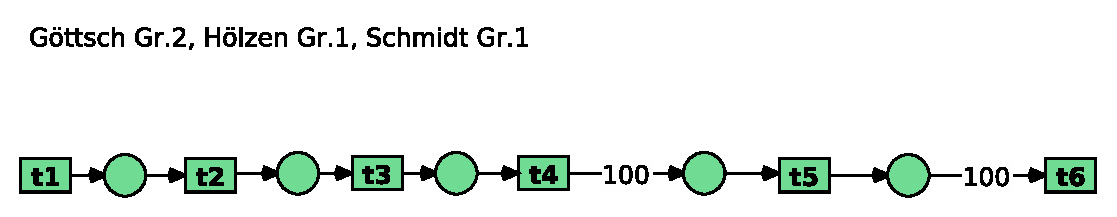
\includegraphics[scale=0.7]{7-5-1.pdf}
\caption{Autofertigung Stufe 1}
\end{figure}

\subsection*{2.}
Im nächsten Verfeinerungsschritt wird der Fertigungsprozess detaillierter modelliert. Dabei ist der vordere Teil des in Abbildung 5 abgebildeten Netzes identisch zum vorherigen, wobei die Transition $t_5$ in zwei Transitionen unterteilt wurde. Die erste der beiden $t_5$ verteilt die Resourcen auf die Arbeitsplätze, wobei vier Marken stellvertretend für vier Reifen auf einen Platz gelegt werden, zwei Marken für zwei Achsen auf einen anderen und jeweils eine Marke für einen Motor und ein Lenkrad auf zwei Plätze. Die Transition $t_6$ modelliert die Montagelinie in der alle Resourcen genommen werden und ein fertiges Produkt in Form einer einzelnen Marke in das Lager gelegt wird.\\

Dieses Netz ist ebenfalls nebenläufig, lebendig und unbeschränkt. Die Argumentation ist dabei die gleiche wie im ersten Schritt. Es ist außerdem auch rücksetzbar, da jede erzeugte Marke auch wieder vernichtet werden kann und so die Startmarkierung wiederherstellbar ist. Die Marken von $t_4$ in $t_7$ und die Marken die von $t_5$ erzeugt werden, werden direkt von $t_6$ wieder entfernt.\\

\begin{figure}[h!]
\centering
\includegraphics[scale=0.7]{7-5-2.pdf}
\caption{Autofertigung Stufe 2}
\end{figure}

\subsection*{3.}
Die nächste Stufe ist in Abbildung 6 zu sehen. Hier ist eine noch kleinschrittigere Modellierung der Produktion gefordert. Der Aufbau ähnelt zu großen Teilen dem des vorherigen Netzes, wobei die Transition $t_6$ in vier einzelne Transitionen geteilt wurde, die die Roboter der Produktionslinie darstellen. Dabei nimmt der erste Roboter $t_6$ zwei Marken (Achsen) von dem Platz, verarbeitet diese und legt sie auf das Fließband, das durch die blauen Plätze modelliert wird. Die vier Plätze veranschaulichen dabei die räumliche Trennung bzw. das Weiterfahren des Bandes. Hier kann $t_7$ nur schalten, wenn $t_6$ ein Teil fertig montiert hat, $t_8$ ist von $t_7$ abhängig und $t_9$ von $t_8$.\\

Das Netz bleibt weiterhin nebenläufig, lebendig und unbeschränkt, dadurch dass die Transition $t_1$ Marken generiert. Außerdem bleibt auch die Rücksetzbarkeit erhalten, da auch in diesem Netz alle Marken, die erzeugt werden, wieder vernichtet werden können.\\

\begin{figure}[h!]
\centering
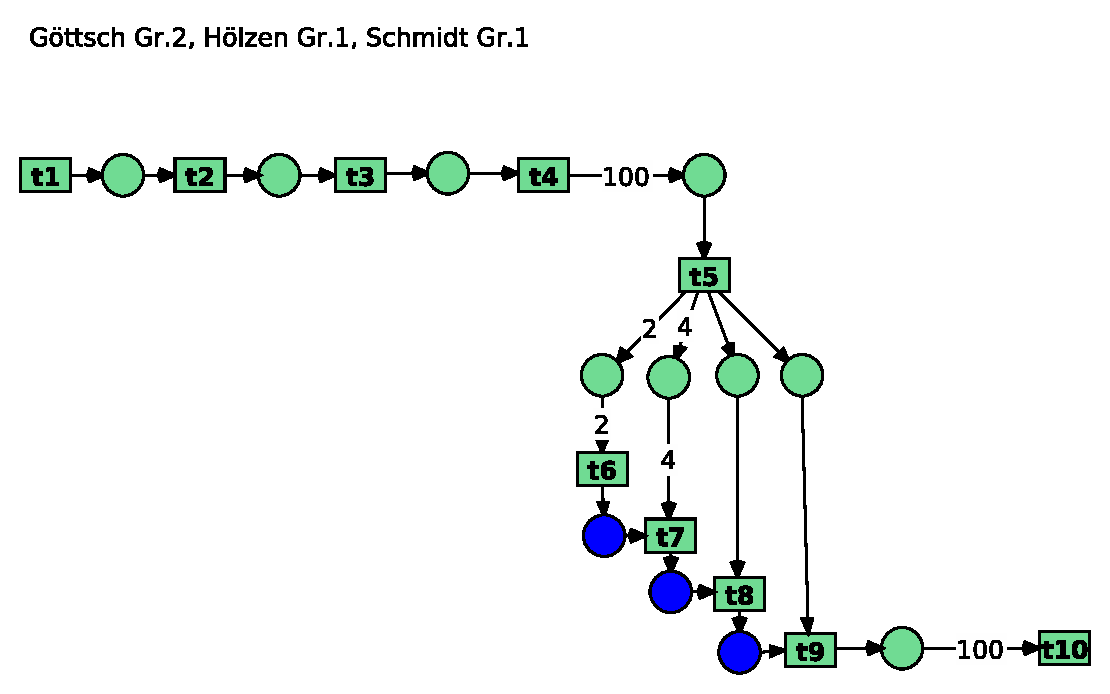
\includegraphics[scale=0.7]{7-5-3.pdf}
\caption{Autofertigung Stufe 3}
\end{figure}

\newpage
\subsection*{4.}
Stufe 4 der Verfeinerung des Netzes führt eine zweite Montagelinie ein. Diese ist durch eine Kopie des entsprechenden Teilnetzes realisiert und in Abbildung 7 zu sehen. Dabei werden die Marken (Resourcen) aus dem gleichen Lager entnommen und die fertigen Produkte in das gleiche Lager gelegt. Die beiden Linien arbeiten voneinander unabhängig.\\

Das Netz besitzt weiterhin Nebenläufigkeit, Lebendigkeit und Unbeschränktheit, sowie Rücksetzbarkeit. Der Determinismus geht jedoch verloren, da die Transitionen $t_5$ und $t_10$ willkürlich geschaltet werden können.\\

\begin{figure}[h!]
\centering
\includegraphics[scale=0.7]{7-5-4.pdf}
\caption{Autofertigung Stufe 4}
\end{figure}

\newpage
\subsection*{5.}
Zum Schluss wird noch ein Konto in das Modell eingeführt, modelliert durch den gelben Platz in Abbildung 8. Er enthält ein Startkapital von 100 Marken, was genau dem Preis für 100 Wagen entspricht, der vom Lieferanten bzw. Transition $t_4$ getilgt wird. Der Spediteur zahlt beim Abholen von 100 PKWs aus dem Lager 200 Marken auf das Konto ein, sodass pro abgeschlossener Bestellung 100 Marken auf dem gelben Platz generiert werden.\\

Das Netz ist nebenläufig, und unbeschränkt, da $t_1$ Marken generiert. Es ist außerdem lebendig, da durch $t_15$ immer genug Marken für die Aktivierung von $t_4$ erzeugt werden können. Es ist weiterhin nicht deterministisch. Die Rücksetzbarkeit des Netzes geht verloren, da auf dem gelben Platz immer mehr Marken generiert werden als vernichtet werden können.\\

\begin{figure}[h!]
\centering
\includegraphics[scale=0.63]{7-5-5.pdf}
\caption{Autofertigung Stufe 5}
\end{figure}

\newpage
\subsection*{6.}
Mögliche Schwächen des Modells sind:
\begin{enumerate}
	\item [1.] Das P/T-Netz ist nicht fair, da es passieren kann, dass z.B. $t_{10}$ niemals schaltet. Das würde bedeuten die Firma \textit{Car Produktion GmbH} würde keinerlei Vorteil aus dem zweiten Montageband ziehen.
	\item [2.] Theoretisch ist es zwar möglich einen Platz mit beliebig vielen Marken zu haben, in der Realität haben Lager aber eine bestimmte Maximalkapazität. Es können also nicht wirklich beliebig viele Aufträge im Eingangsfach liegen oder unendlich viele Autoteile in einem Lager.
\end{enumerate}

\end{document}
